\chapter{Results}

\section{Speed measurements}

\par
Actual speed measurement is performed within \emph{GenerateData} method of the FiniteDifferenceFilter.
Counter is started right after initialization phase (i.e. before main algorithm loop) and stopped right after the loop.
Program memory usage was tuned to use only really necessary amount of memory within measured interval.
Valgrind's massive tool was used for the memory usage tuning.
This was necessary because of the PS3 small memory and because we want to leave swap file untouched during the speed measurement.

\par
Meanwhile this server memory usage tunning some changes was made also within client part.
There was special filter developped.
That filter shrings dataset to given size and cast its voxels to float.
Shrinking is performed by linear interpolation.
The purpose of the float casting is avoiding allocation of additional memory to perform it on the server side.

//TODO popsat ze to mozna nemelo cenu, protoze top stejne ukazuje pres 100Mega kdyz to bezi
\par
Results of the speed measurement is summarized within Table \ref{tab:runresults}.

\begin{table}
\centering
\begin{tabular}{|c|c|c|c|}
\hline
\multicolumn{4}{|c|}{Measurement results}\\
\hline
Data set&Architecture&time spend&percent\\&&in calculations&\%\\&&(in seconds)&\\
\hline
\hline
ApplyUpdate()	&				&	20.15&	75.21\\
\hline
		&PropagateAllLayerValues()	&	16.64&	62.11\\
\hline
		&UpdateActiveLayerValues()	&	2.27&	8.47\\
\hline
CalculateChange()&				&	6.11&	22.8\\
\hline
		&ComputeUpdate()		&	3.97&	14.82\\
\hline
TOTAL		&				&	26.79&	100\\
\hline
\end{tabular}
\par
\caption[Measurement results]
{
  Results of speed measurement //TODO
}
\label{tab:runresults}
\end{table}

\section{Pictures}

\section{Reasons of slowdown and possible improvements}

\par
Porting the code to run on SPEs is not sufficient to get more speed from Cell B.E. over traditional processors.
Aditional speedup porting phases are necessary.
But our program has another speed pitfalls.

\par
The biggest of them is CellNeighbourhood that represent small segment of an image (the $3^3$ voxel matrix).
It is transferred for every layer (linked chain of nodes) item.
In some parts the both output and status image neighbourhoods are transfered.
We wanted to perform the transfer in scatter-geather manner through the DMA lists but we have faced some problems concerning this way of transfer.
The DMA transfers (and specially using DMA lists) are designed for bigger amount of aligned data.
When used for small amounts (smaller that 16bytes per list item) performance goes down because transfer of unaligned data.
When data smaller than 16 bytes (quadword) are being transferred, every single item is automatically aligned to quadword address within local store buffer (see Figure \ref{fg:automaticAlignOfSmallData}).

\begin{figure}
    \centering
    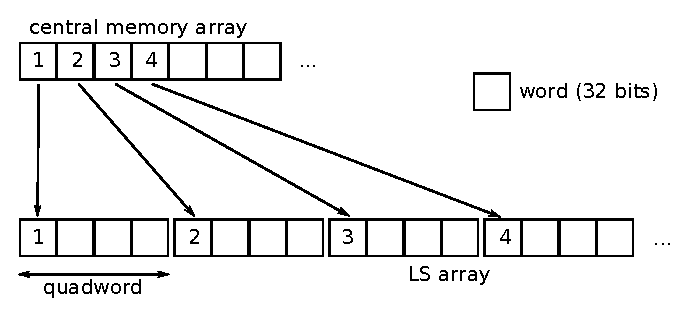
\includegraphics[width=0.5\textwidth]{data/automaticAlignOfSmallData}
    \caption[automatic align of small data]
{
  Illustration of transfer of data that are smaller that quadword.
  Hardware automatically increase address within local store buffer in such way that every transferred item is quadword aligned.
}
    \label{fg:automaticAlignOfSmallData}
\end{figure}

This increase required size of buffer that is needed for the transfer.
This can be partially solved by usage of multiple DMA lists (one for each quadword align).
This is illustrated on Figure \ref{fg:multipleDMAList}.
For details see \cite{DMAListIssues}.

\begin{figure}
    \centering
    \includegraphics[width=0.5\textwidth]{data/multipleDMAList}
    \caption[multiple DMA list workaround]
{
  Workaround for transfer in smaller than quadword chunks.
  Uses more that one DMA list.
  One per quadword align (e.g. for single bytes 16 DMA lists are needed).
}
    \label{fg:multipleDMAList}
\end{figure}

We have adopted this workaround and used it within the neigbourhood transfer.
Because if automatic local store quadword address aligning we had to use a translation table that maps position of actual neigbourhood members into the local store buffer which had to be enlarged appropriately based on data type that stores.
This is functional solution but overhead for SPE is increadible.

\par
Another problem is order of layer nodes (and thus neigbourhoods) processing.
When there are two nodes within one layer that are next to each other and processed subsequently.
Changes made to the first processed neigbourhood would not appear to already preloaded next one.
So another merging need to be performed.

\par
This coerced another changes to neighbourhood tranfer and made the actual transfer unbearably expensive operation.

\par
Aditional pitfall is the situation when sibling nodes are processed by two different SPEs.
Adding nodes to layers is based on information from currently processed node's neighbours.
So it is possible that two different SPE inserts the same nodes more time into one layer because they process sibling nodes (i.e. overlapping neighbourhhods).
This makes no changes to output but aditional overhead due to processing multiplied nodes.
Solution to this problem would be synchronization among the SPEs.

\par
To speed up the execution improvement of neighbourhood transfers should be done.
This corresponds to data trasfer optimization step of porting process (see \ref{fg:appPorting})
In our case this means radical simplification of neighbourhood transfers.
This means utilisation of bigger DMA tranfers

total redesign of node processing to utilize spatial information of node when inserted into a layer

// ze data z 1 okoli moji prunik z uz naloadovanymi a zmeny se musi mergovat.=> idealni zpracovava nezavisle chunky
//popsat rezii prenaseni okoli, na todle ze to je naprd
// popsat jake jsou moznosti na zrychleni a co proto je treba udelat.
// popsat porting process podle me, ze nejdriv rozmyslet a kdyz je moc velka rezie na predos dat, tak to nema ani cenu implementovat

// popsat proc todle neni algoritmus, ktery je krasne zrychlitelny a uvest protipriklad. Treba tresholding?

\section{Code and design complexity}
// porovnat slozitost kodu a navrhu

\section{Algorithm complexity}

\par
The implemented algorithm is complex enough to be offloaded to compute on remote mashine.
It is tradeoff between time spent in transfer of actual dataset and the time we spare with computation on better hardware.
E.g. simple thresholding would be worthless to compute remotely because the overhead of data trasfer to another mashine.

\par
But the nature of the thresholding is exactly targeted for streaming architecture such as Cell B.E..
So as soon as common machines such as notebooks, desktops are equipped with the Cell B.E. processor even class of such simple image processing algorithms (such as the thresholding or variety of masking, edge detections) that is implemented in everyday-use software could take advantage of the processor.
But nowadays is available only in Blade servers and PS3 so only such complex algorithms like e.g. level sets are worth to port.
We think the pallet of tools and features of the Cell B.E. can make it well suited for every algorithm.
Some of the algorithms suits more and the performance gain is huge.
But for some of them could not suit as well so usage of another technique (another data structure or different transfer scheme) is needed.
Of course there is a question if all the efforts are worth the results. //TODO

\chapter{Conclusion}

At the beginning we studied available literature to find out what is actually Cell B.E., what benefits it brings for what price.
What special features it have and what are they good for.
Then we have been trying to install SDK to start actual development process.
During this phase we faced some obstacles like bugs, incompatibilities among tools, libraries that the tools use and even operating system vs. SDK incompatibilities.
So we had to go through variety of forums and other sources to find the solution.
As a side effect we improved our Linux knowledge.
Eventually we managed to install SDK and was able to start developing.
Then we tested variety of libraries, tools and other feature that the SDK brings.
We have chosen level set based segmentation algorithm implementing sparse field accelerating method to port to Cell B.E. platform.
This is quite complex algorithm to test the platform's potential.
We adopted ITK implementation of that algorithm.
So we had to study ITK toolkit and its internals.
We have also incorporated the whole program into MedV4D framework.
That means we have implemented some new modules that allows using ITK and can offload some part of processing to another machine (that run on Cell B.E.).
Actual porting process started with profiling of existing application.
This step have found out hot spots of the code which can be in turn offloaded to SPE to take advantage of Cell B.E. potential.
But results was qiote unexpected so another redesign of application followed.
In this new design almost whole original ITK pipeline was offloaded into SPE.
Big code restructuralisation was necessary to allow to perform actual computations on SPE.
Finnaly we have able to run the whole algorithm on SPE and thus to measure time need for computations.
The result of measurement showed that simple move the computation to SPE slows down the computations so when one want to take advantages of Cell B.E. potential another code optimalisations should be performed.
We have proposed some optimalisations that could increase the performance of our application.

\par
The Cell B.E. platform is very interresting for its variations of use scenarios and ability of program tuning and customization.
We think its great potential has already been proven.
But it is still waiting for wider spectrum of programmers.

\par
If the process of starting developing on Cell B.E. would become simplier we belive much more new programmers would be start.
Nowadays there are plenty of information about Cell B.E. but somehow unsorted or out of date.
The best information source are documents shipped along the SDK.
But they are targetted to contain all the information regardless the level of experience of the reader.
So when a programmer wants to start developing applications on Cell B.E. he would go trough plenty of that information before he can start actual work.
It's a pity there are total lack of information for PS3 users within SDK docs.
This is quite problem when big part of begginers has PS3 available.
There is simply lack of some "cookbook for beginners" with practical information and some howtos.
We believe is such cookbook with some of practical information that potentially may help to some other programmers who would like to start developing for Cell B.E.